\documentclass[1p]{elsarticle_modified}
%\bibliographystyle{elsarticle-num}

%\usepackage[colorlinks]{hyperref}
%\usepackage{abbrmath_seonhwa} %\Abb, \Ascr, \Acal ,\Abf, \Afrak
\usepackage{amsfonts}
\usepackage{amssymb}
\usepackage{amsmath}
\usepackage{amsthm}
\usepackage{scalefnt}
\usepackage{amsbsy}
\usepackage{kotex}
\usepackage{caption}
\usepackage{subfig}
\usepackage{color}
\usepackage{graphicx}
\usepackage{xcolor} %% white, black, red, green, blue, cyan, magenta, yellow
\usepackage{float}
\usepackage{setspace}
\usepackage{hyperref}

\usepackage{tikz}
\usetikzlibrary{arrows}

\usepackage{multirow}
\usepackage{array} % fixed length table
\usepackage{hhline}

%%%%%%%%%%%%%%%%%%%%%
\makeatletter
\renewcommand*\env@matrix[1][\arraystretch]{%
	\edef\arraystretch{#1}%
	\hskip -\arraycolsep
	\let\@ifnextchar\new@ifnextchar
	\array{*\c@MaxMatrixCols c}}
\makeatother %https://tex.stackexchange.com/questions/14071/how-can-i-increase-the-line-spacing-in-a-matrix
%%%%%%%%%%%%%%%

\usepackage[normalem]{ulem}

\newcommand{\msout}[1]{\ifmmode\text{\sout{\ensuremath{#1}}}\else\sout{#1}\fi}
%SOURCE: \msout is \stkout macro in https://tex.stackexchange.com/questions/20609/strikeout-in-math-mode

\newcommand{\cancel}[1]{
	\ifmmode
	{\color{red}\msout{#1}}
	\else
	{\color{red}\sout{#1}}
	\fi
}

\newcommand{\add}[1]{
	{\color{blue}\uwave{#1}}
}

\newcommand{\replace}[2]{
	\ifmmode
	{\color{red}\msout{#1}}{\color{blue}\uwave{#2}}
	\else
	{\color{red}\sout{#1}}{\color{blue}\uwave{#2}}
	\fi
}

\newcommand{\Sol}{\mathcal{S}} %segment
\newcommand{\D}{D} %diagram
\newcommand{\A}{\mathcal{A}} %arc


%%%%%%%%%%%%%%%%%%%%%%%%%%%%%5 test

\def\sl{\operatorname{\textup{SL}}(2,\Cbb)}
\def\psl{\operatorname{\textup{PSL}}(2,\Cbb)}
\def\quan{\mkern 1mu \triangleright \mkern 1mu}

\theoremstyle{definition}
\newtheorem{thm}{Theorem}[section]
\newtheorem{prop}[thm]{Proposition}
\newtheorem{lem}[thm]{Lemma}
\newtheorem{ques}[thm]{Question}
\newtheorem{cor}[thm]{Corollary}
\newtheorem{defn}[thm]{Definition}
\newtheorem{exam}[thm]{Example}
\newtheorem{rmk}[thm]{Remark}
\newtheorem{alg}[thm]{Algorithm}

\newcommand{\I}{\sqrt{-1}}
\begin{document}

%\begin{frontmatter}
%
%\title{Boundary parabolic representations of knots up to 8 crossings}
%
%%% Group authors per affiliation:
%\author{Yunhi Cho} 
%\address{Department of Mathematics, University of Seoul, Seoul, Korea}
%\ead{yhcho@uos.ac.kr}
%
%
%\author{Seonhwa Kim} %\fnref{s_kim}}
%\address{Center for Geometry and Physics, Institute for Basic Science, Pohang, 37673, Korea}
%\ead{ryeona17@ibs.re.kr}
%
%\author{Hyuk Kim}
%\address{Department of Mathematical Sciences, Seoul National University, Seoul 08826, Korea}
%\ead{hyukkim@snu.ac.kr}
%
%\author{Seokbeom Yoon}
%\address{Department of Mathematical Sciences, Seoul National University, Seoul, 08826,  Korea}
%\ead{sbyoon15@snu.ac.kr}
%
%\begin{abstract}
%We find all boundary parabolic representation of knots up to 8 crossings.
%
%\end{abstract}
%\begin{keyword}
%    \MSC[2010] 57M25 
%\end{keyword}
%
%\end{frontmatter}

%\linenumbers
%\tableofcontents
%
\newcommand\colored[1]{\textcolor{white}{\rule[-0.35ex]{0.8em}{1.4ex}}\kern-0.8em\color{red} #1}%
%\newcommand\colored[1]{\textcolor{white}{ #1}\kern-2.17ex	\textcolor{white}{ #1}\kern-1.81ex	\textcolor{white}{ #1}\kern-2.15ex\color{red}#1	}

{\Large $\underline{12a_{0255}~(K12a_{0255})}$}

\setlength{\tabcolsep}{10pt}
\renewcommand{\arraystretch}{1.6}
\vspace{1cm}\begin{tabular}{m{100pt}>{\centering\arraybackslash}m{274pt}}
\multirow{5}{120pt}{
	\centering
	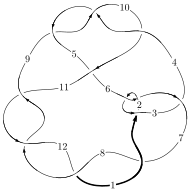
\includegraphics[width=112pt]{../../../GIT/diagram.site/Diagrams/png/1056_12a_0255.png}\\
\ \ \ A knot diagram\footnotemark}&
\allowdisplaybreaks
\textbf{Linearized knot diagam} \\
\cline{2-2}
 &
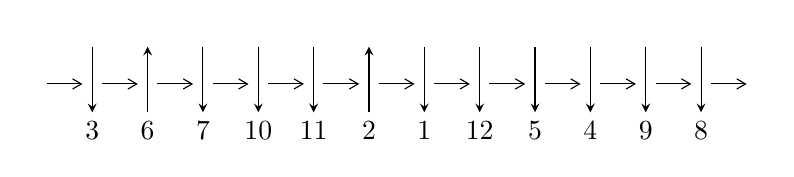
\begin{tikzpicture}[x=20pt, y=17pt]
	% nodes
	\node (C0) at (0, 0) {};
	\node (C1) at (1, 0) {};
	\node (C1U) at (1, +1) {};
	\node (C1D) at (1, -1) {3};

	\node (C2) at (2, 0) {};
	\node (C2U) at (2, +1) {};
	\node (C2D) at (2, -1) {6};

	\node (C3) at (3, 0) {};
	\node (C3U) at (3, +1) {};
	\node (C3D) at (3, -1) {7};

	\node (C4) at (4, 0) {};
	\node (C4U) at (4, +1) {};
	\node (C4D) at (4, -1) {10};

	\node (C5) at (5, 0) {};
	\node (C5U) at (5, +1) {};
	\node (C5D) at (5, -1) {11};

	\node (C6) at (6, 0) {};
	\node (C6U) at (6, +1) {};
	\node (C6D) at (6, -1) {2};

	\node (C7) at (7, 0) {};
	\node (C7U) at (7, +1) {};
	\node (C7D) at (7, -1) {1};

	\node (C8) at (8, 0) {};
	\node (C8U) at (8, +1) {};
	\node (C8D) at (8, -1) {12};

	\node (C9) at (9, 0) {};
	\node (C9U) at (9, +1) {};
	\node (C9D) at (9, -1) {5};

	\node (C10) at (10, 0) {};
	\node (C10U) at (10, +1) {};
	\node (C10D) at (10, -1) {4};

	\node (C11) at (11, 0) {};
	\node (C11U) at (11, +1) {};
	\node (C11D) at (11, -1) {9};

	\node (C12) at (12, 0) {};
	\node (C12U) at (12, +1) {};
	\node (C12D) at (12, -1) {8};
	\node (C13) at (13, 0) {};

	% arrows
	\draw[->,>={angle 60}]
	(C0) edge (C1) (C1) edge (C2) (C2) edge (C3) (C3) edge (C4) (C4) edge (C5) (C5) edge (C6) (C6) edge (C7) (C7) edge (C8) (C8) edge (C9) (C9) edge (C10) (C10) edge (C11) (C11) edge (C12) (C12) edge (C13) ;	\draw[->,>=stealth]
	(C1U) edge (C1D) (C2D) edge (C2U) (C3U) edge (C3D) (C4U) edge (C4D) (C5U) edge (C5D) (C6D) edge (C6U) (C7U) edge (C7D) (C8U) edge (C8D) (C9U) edge (C9D) (C10U) edge (C10D) (C11U) edge (C11D) (C12U) edge (C12D) ;
	\end{tikzpicture} \\
\hhline{~~} \\& 
\textbf{Solving Sequence} \\ \cline{2-2} 
 &
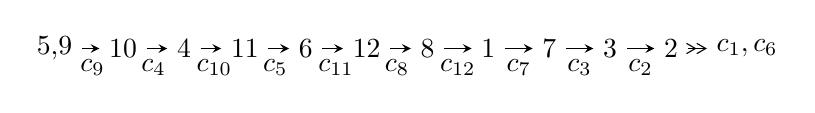
\begin{tikzpicture}[x=22pt, y=7pt]
	% node
	\node (A0) at (-1/8, 0) {5,9};
	\node (A1) at (1, 0) {10};
	\node (A2) at (2, 0) {4};
	\node (A3) at (3, 0) {11};
	\node (A4) at (4, 0) {6};
	\node (A5) at (5, 0) {12};
	\node (A6) at (6, 0) {8};
	\node (A7) at (7, 0) {1};
	\node (A8) at (8, 0) {7};
	\node (A9) at (9, 0) {3};
	\node (A10) at (10, 0) {2};
	\node (C1) at (1/2, -1) {$c_{9}$};
	\node (C2) at (3/2, -1) {$c_{4}$};
	\node (C3) at (5/2, -1) {$c_{10}$};
	\node (C4) at (7/2, -1) {$c_{5}$};
	\node (C5) at (9/2, -1) {$c_{11}$};
	\node (C6) at (11/2, -1) {$c_{8}$};
	\node (C7) at (13/2, -1) {$c_{12}$};
	\node (C8) at (15/2, -1) {$c_{7}$};
	\node (C9) at (17/2, -1) {$c_{3}$};
	\node (C10) at (19/2, -1) {$c_{2}$};
	\node (A11) at (45/4, 0) {$c_{1},c_{6}$};

	% edge
	\draw[->,>=stealth]	
	(A0) edge (A1) (A1) edge (A2) (A2) edge (A3) (A3) edge (A4) (A4) edge (A5) (A5) edge (A6) (A6) edge (A7) (A7) edge (A8) (A8) edge (A9) (A9) edge (A10) ;
	\draw[->>,>={angle 60}]	
	(A10) edge (A11);
\end{tikzpicture} \\ 

\end{tabular} \\

\footnotetext{
The image of knot diagram is generated by the software ``\textbf{Draw programme}" developed by Andrew Bartholomew(\url{http://www.layer8.co.uk/maths/draw/index.htm\#Running-draw}), where we modified some parts for our purpose(\url{https://github.com/CATsTAILs/LinksPainter}).
}\phantom \\ \newline 
\centering \textbf{Ideals for irreducible components\footnotemark of $X_{\text{par}}$} 
 
\begin{align*}
I^u_{1}&=\langle 
u^{53}+u^{52}+\cdots+u-1\rangle \\
\\
\end{align*}
\raggedright * 1 irreducible components of $\dim_{\mathbb{C}}=0$, with total 53 representations.\\
\footnotetext{All coefficients of polynomials are rational numbers. But the coefficients are sometimes approximated in decimal forms when there is not enough margin.}
\newpage
\renewcommand{\arraystretch}{1}
\centering \section*{I. $I^u_{1}= \langle u^{53}+u^{52}+\cdots+u-1 \rangle$}
\flushleft \textbf{(i) Arc colorings}\\
\begin{tabular}{m{7pt} m{180pt} m{7pt} m{180pt} }
\flushright $a_{5}=$&$\begin{pmatrix}0\\u\end{pmatrix}$ \\
\flushright $a_{9}=$&$\begin{pmatrix}1\\0\end{pmatrix}$ \\
\flushright $a_{10}=$&$\begin{pmatrix}1\\u^2\end{pmatrix}$ \\
\flushright $a_{4}=$&$\begin{pmatrix}u\\u^3+u\end{pmatrix}$ \\
\flushright $a_{11}=$&$\begin{pmatrix}u^2+1\\u^4+2 u^2\end{pmatrix}$ \\
\flushright $a_{6}=$&$\begin{pmatrix}- u^5-2 u^3- u\\- u^7-3 u^5-2 u^3+u\end{pmatrix}$ \\
\flushright $a_{12}=$&$\begin{pmatrix}- u^4- u^2+1\\u^4+2 u^2\end{pmatrix}$ \\
\flushright $a_{8}=$&$\begin{pmatrix}u^8+3 u^6+u^4-2 u^2+1\\- u^8-4 u^6-4 u^4\end{pmatrix}$ \\
\flushright $a_{1}=$&$\begin{pmatrix}- u^{12}-5 u^{10}-7 u^8+2 u^4-3 u^2+1\\u^{12}+6 u^{10}+12 u^8+8 u^6+u^4+2 u^2\end{pmatrix}$ \\
\flushright $a_{7}=$&$\begin{pmatrix}u^{16}+7 u^{14}+17 u^{12}+14 u^{10}- u^8+2 u^6+6 u^4-4 u^2+1\\- u^{16}-8 u^{14}-24 u^{12}-32 u^{10}-18 u^8-8 u^6-8 u^4\end{pmatrix}$ \\
\flushright $a_{3}=$&$\begin{pmatrix}u^{35}+16 u^{33}+\cdots-7 u^3+2 u\\- u^{35}-17 u^{33}+\cdots+u^3+u\end{pmatrix}$ \\
\flushright $a_{2}=$&$\begin{pmatrix}u^{47}+22 u^{45}+\cdots-10 u^3+2 u\\u^{49}+23 u^{47}+\cdots+4 u^3+u\end{pmatrix}$\\&\end{tabular}
\flushleft \textbf{(ii) Obstruction class $= -1$}\\~\\
\flushleft \textbf{(iii) Cusp Shapes $= -4 u^{51}-4 u^{50}+\cdots+4 u-10$}\\~\\
\newpage\renewcommand{\arraystretch}{1}
\flushleft \textbf{(iv) u-Polynomials at the component}\newline \\
\begin{tabular}{m{50pt}|m{274pt}}
Crossings & \hspace{64pt}u-Polynomials at each crossing \\
\hline $$\begin{aligned}c_{1}\end{aligned}$$&$\begin{aligned}
&u^{53}+23 u^{52}+\cdots+3 u-1
\end{aligned}$\\
\hline $$\begin{aligned}c_{2},c_{6}\end{aligned}$$&$\begin{aligned}
&u^{53}- u^{52}+\cdots- u+1
\end{aligned}$\\
\hline $$\begin{aligned}c_{3}\end{aligned}$$&$\begin{aligned}
&u^{53}+u^{52}+\cdots+25 u+5
\end{aligned}$\\
\hline $$\begin{aligned}c_{4},c_{9},c_{10}\end{aligned}$$&$\begin{aligned}
&u^{53}- u^{52}+\cdots+u+1
\end{aligned}$\\
\hline $$\begin{aligned}c_{5}\end{aligned}$$&$\begin{aligned}
&u^{53}+u^{52}+\cdots+3303 u+1237
\end{aligned}$\\
\hline $$\begin{aligned}c_{7},c_{8},c_{11}\\c_{12}\end{aligned}$$&$\begin{aligned}
&u^{53}-5 u^{52}+\cdots-43 u+3
\end{aligned}$\\
\hline
\end{tabular}\\~\\
\newpage\renewcommand{\arraystretch}{1}
\flushleft \textbf{(v) Riley Polynomials at the component}\newline \\
\begin{tabular}{m{50pt}|m{274pt}}
Crossings & \hspace{64pt}Riley Polynomials at each crossing \\
\hline $$\begin{aligned}c_{1}\end{aligned}$$&$\begin{aligned}
&y^{53}+15 y^{52}+\cdots+43 y-1
\end{aligned}$\\
\hline $$\begin{aligned}c_{2},c_{6}\end{aligned}$$&$\begin{aligned}
&y^{53}+23 y^{52}+\cdots+3 y-1
\end{aligned}$\\
\hline $$\begin{aligned}c_{3}\end{aligned}$$&$\begin{aligned}
&y^{53}+7 y^{52}+\cdots-65 y-25
\end{aligned}$\\
\hline $$\begin{aligned}c_{4},c_{9},c_{10}\end{aligned}$$&$\begin{aligned}
&y^{53}+51 y^{52}+\cdots+3 y-1
\end{aligned}$\\
\hline $$\begin{aligned}c_{5}\end{aligned}$$&$\begin{aligned}
&y^{53}+31 y^{52}+\cdots-35851265 y-1530169
\end{aligned}$\\
\hline $$\begin{aligned}c_{7},c_{8},c_{11}\\c_{12}\end{aligned}$$&$\begin{aligned}
&y^{53}+67 y^{52}+\cdots-41 y-9
\end{aligned}$\\
\hline
\end{tabular}\\~\\
\newpage\flushleft \textbf{(vi) Complex Volumes and Cusp Shapes}
$$\begin{array}{c|c|c}  
\text{Solutions to }I^u_{1}& \I (\text{vol} + \sqrt{-1}CS) & \text{Cusp shape}\\
 \hline 
\begin{aligned}
u &= \phantom{-}0.681869 + 0.507223 I\end{aligned}
 & \phantom{-}11.40680 - 0.55910 I & -1.54942 + 2.72992 I \\ \hline\begin{aligned}
u &= \phantom{-}0.681869 - 0.507223 I\end{aligned}
 & \phantom{-}11.40680 + 0.55910 I & -1.54942 - 2.72992 I \\ \hline\begin{aligned}
u &= -0.676067 + 0.514665 I\end{aligned}
 & \phantom{-}9.65619 - 4.88920 I & -3.91750 + 1.84392 I \\ \hline\begin{aligned}
u &= -0.676067 - 0.514665 I\end{aligned}
 & \phantom{-}9.65619 + 4.88920 I & -3.91750 - 1.84392 I \\ \hline\begin{aligned}
u &= \phantom{-}0.694473 + 0.488863 I\end{aligned}
 & \phantom{-}11.34170 - 4.02382 I & -1.72591 + 3.04100 I \\ \hline\begin{aligned}
u &= \phantom{-}0.694473 - 0.488863 I\end{aligned}
 & \phantom{-}11.34170 + 4.02382 I & -1.72591 - 3.04100 I \\ \hline\begin{aligned}
u &= -0.699005 + 0.481452 I\end{aligned}
 & \phantom{-}9.53833 + 9.46936 I & -4.26043 - 7.54800 I \\ \hline\begin{aligned}
u &= -0.699005 - 0.481452 I\end{aligned}
 & \phantom{-}9.53833 - 9.46936 I & -4.26043 + 7.54800 I \\ \hline\begin{aligned}
u &= -0.673401 + 0.486673 I\end{aligned}
 & \phantom{-}5.56712 + 2.23678 I & -7.47397 - 2.96653 I \\ \hline\begin{aligned}
u &= -0.673401 - 0.486673 I\end{aligned}
 & \phantom{-}5.56712 - 2.23678 I & -7.47397 + 2.96653 I \\ \hline\begin{aligned}
u &= -0.070592 + 1.229840 I\end{aligned}
 & \phantom{-}0.281107 - 0.892679 I & \phantom{-0.000000 } 0 \\ \hline\begin{aligned}
u &= -0.070592 - 1.229840 I\end{aligned}
 & \phantom{-}0.281107 + 0.892679 I & \phantom{-0.000000 } 0 \\ \hline\begin{aligned}
u &= -0.143523 + 1.274530 I\end{aligned}
 & \phantom{-}1.01818 + 5.73685 I & \phantom{-0.000000 } 0 \\ \hline\begin{aligned}
u &= -0.143523 - 1.274530 I\end{aligned}
 & \phantom{-}1.01818 - 5.73685 I & \phantom{-0.000000 } 0 \\ \hline\begin{aligned}
u &= \phantom{-}0.097467 + 1.303840 I\end{aligned}
 & \phantom{-}3.26132 - 1.87247 I & \phantom{-0.000000 } 0 \\ \hline\begin{aligned}
u &= \phantom{-}0.097467 - 1.303840 I\end{aligned}
 & \phantom{-}3.26132 + 1.87247 I & \phantom{-0.000000 } 0 \\ \hline\begin{aligned}
u &= \phantom{-}0.603468 + 0.311061 I\end{aligned}
 & \phantom{-}0.37156 - 7.12755 I & -7.47939 + 9.71650 I \\ \hline\begin{aligned}
u &= \phantom{-}0.603468 - 0.311061 I\end{aligned}
 & \phantom{-}0.37156 + 7.12755 I & -7.47939 - 9.71650 I \\ \hline\begin{aligned}
u &= -0.564862 + 0.337345 I\end{aligned}
 & \phantom{-}2.18676 + 2.45806 I & -3.45434 - 5.09899 I \\ \hline\begin{aligned}
u &= -0.564862 - 0.337345 I\end{aligned}
 & \phantom{-}2.18676 - 2.45806 I & -3.45434 + 5.09899 I \\ \hline\begin{aligned}
u &= \phantom{-}0.421531 + 0.474326 I\end{aligned}
 & \phantom{-}1.11217 + 3.72638 I & -4.30676 - 2.36666 I \\ \hline\begin{aligned}
u &= \phantom{-}0.421531 - 0.474326 I\end{aligned}
 & \phantom{-}1.11217 - 3.72638 I & -4.30676 + 2.36666 I \\ \hline\begin{aligned}
u &= -0.473604 + 0.418047 I\end{aligned}
 & \phantom{-}2.56522 + 0.88236 I & -1.57464 - 3.79176 I \\ \hline\begin{aligned}
u &= -0.473604 - 0.418047 I\end{aligned}
 & \phantom{-}2.56522 - 0.88236 I & -1.57464 + 3.79176 I \\ \hline\begin{aligned}
u &= \phantom{-}0.180145 + 1.378190 I\end{aligned}
 & \phantom{-}3.35085 - 3.35943 I & \phantom{-0.000000 } 0 \\ \hline\begin{aligned}
u &= \phantom{-}0.180145 - 1.378190 I\end{aligned}
 & \phantom{-}3.35085 + 3.35943 I & \phantom{-0.000000 } 0 \\ \hline\begin{aligned}
u &= \phantom{-}0.026399 + 1.391270 I\end{aligned}
 & \phantom{-}4.96113 - 2.14784 I & \phantom{-0.000000 } 0 \\ \hline\begin{aligned}
u &= \phantom{-}0.026399 - 1.391270 I\end{aligned}
 & \phantom{-}4.96113 + 2.14784 I & \phantom{-0.000000 } 0 \\ \hline\begin{aligned}
u &= \phantom{-}0.535008 + 0.220142 I\end{aligned}
 & -1.72716 - 0.77447 I & -12.25842 + 4.43698 I \\ \hline\begin{aligned}
u &= \phantom{-}0.535008 - 0.220142 I\end{aligned}
 & -1.72716 + 0.77447 I & -12.25842 - 4.43698 I\\
 \hline 
 \end{array}$$\newpage$$\begin{array}{c|c|c}  
\text{Solutions to }I^u_{1}& \I (\text{vol} + \sqrt{-1}CS) & \text{Cusp shape}\\
 \hline 
\begin{aligned}
u &= \phantom{-}0.21720 + 1.40718 I\end{aligned}
 & \phantom{-}5.84972 - 10.11280 I & \phantom{-0.000000 } 0 \\ \hline\begin{aligned}
u &= \phantom{-}0.21720 - 1.40718 I\end{aligned}
 & \phantom{-}5.84972 + 10.11280 I & \phantom{-0.000000 } 0 \\ \hline\begin{aligned}
u &= -0.20092 + 1.41590 I\end{aligned}
 & \phantom{-}7.78346 + 5.25251 I & \phantom{-0.000000 } 0 \\ \hline\begin{aligned}
u &= -0.20092 - 1.41590 I\end{aligned}
 & \phantom{-}7.78346 - 5.25251 I & \phantom{-0.000000 } 0 \\ \hline\begin{aligned}
u &= -0.555680 + 0.056230 I\end{aligned}
 & -3.01508 + 3.19278 I & -15.3921 - 5.6502 I \\ \hline\begin{aligned}
u &= -0.555680 - 0.056230 I\end{aligned}
 & -3.01508 - 3.19278 I & -15.3921 + 5.6502 I \\ \hline\begin{aligned}
u &= -0.16103 + 1.43665 I\end{aligned}
 & \phantom{-}8.48816 + 3.19971 I & \phantom{-0.000000 } 0 \\ \hline\begin{aligned}
u &= -0.16103 - 1.43665 I\end{aligned}
 & \phantom{-}8.48816 - 3.19971 I & \phantom{-0.000000 } 0 \\ \hline\begin{aligned}
u &= \phantom{-}0.13893 + 1.44337 I\end{aligned}
 & \phantom{-}7.20577 + 1.69986 I & \phantom{-0.000000 } 0 \\ \hline\begin{aligned}
u &= \phantom{-}0.13893 - 1.44337 I\end{aligned}
 & \phantom{-}7.20577 - 1.69986 I & \phantom{-0.000000 } 0 \\ \hline\begin{aligned}
u &= -0.23600 + 1.49454 I\end{aligned}
 & \phantom{-}11.99430 + 5.55348 I & \phantom{-0.000000 } 0 \\ \hline\begin{aligned}
u &= -0.23600 - 1.49454 I\end{aligned}
 & \phantom{-}11.99430 - 5.55348 I & \phantom{-0.000000 } 0 \\ \hline\begin{aligned}
u &= -0.24698 + 1.49787 I\end{aligned}
 & \phantom{-}15.9616 + 12.9219 I & \phantom{-0.000000 } 0 \\ \hline\begin{aligned}
u &= -0.24698 - 1.49787 I\end{aligned}
 & \phantom{-}15.9616 - 12.9219 I & \phantom{-0.000000 } 0 \\ \hline\begin{aligned}
u &= \phantom{-}0.24357 + 1.49991 I\end{aligned}
 & \phantom{-}17.8000 - 7.4463 I & \phantom{-0.000000 } 0 \\ \hline\begin{aligned}
u &= \phantom{-}0.24357 - 1.49991 I\end{aligned}
 & \phantom{-}17.8000 + 7.4463 I & \phantom{-0.000000 } 0 \\ \hline\begin{aligned}
u &= \phantom{-}0.23418 + 1.50440 I\end{aligned}
 & \phantom{-}17.9500 - 3.8966 I & \phantom{-0.000000 } 0 \\ \hline\begin{aligned}
u &= \phantom{-}0.23418 - 1.50440 I\end{aligned}
 & \phantom{-}17.9500 + 3.8966 I & \phantom{-0.000000 } 0 \\ \hline\begin{aligned}
u &= -0.22997 + 1.50583 I\end{aligned}
 & \phantom{-}16.2324 - 1.5914 I & \phantom{-0.000000 } 0 \\ \hline\begin{aligned}
u &= -0.22997 - 1.50583 I\end{aligned}
 & \phantom{-}16.2324 + 1.5914 I & \phantom{-0.000000 } 0 \\ \hline\begin{aligned}
u &= \phantom{-}0.138924 + 0.415337 I\end{aligned}
 & -0.51035 - 1.61303 I & -4.76097 + 3.99384 I \\ \hline\begin{aligned}
u &= \phantom{-}0.138924 - 0.415337 I\end{aligned}
 & -0.51035 + 1.61303 I & -4.76097 - 3.99384 I \\ \hline\begin{aligned}
u &= \phantom{-}0.436950\phantom{ +0.000000I}\end{aligned}
 & -0.761067\phantom{ +0.000000I} & -12.9280\phantom{ +0.000000I}\\
 \hline 
 \end{array}$$\newpage
\newpage\renewcommand{\arraystretch}{1}
\centering \section*{ II. u-Polynomials}
\begin{tabular}{m{50pt}|m{274pt}}
Crossings & \hspace{64pt}u-Polynomials at each crossing \\
\hline $$\begin{aligned}c_{1}\end{aligned}$$&$\begin{aligned}
&u^{53}+23 u^{52}+\cdots+3 u-1
\end{aligned}$\\
\hline $$\begin{aligned}c_{2},c_{6}\end{aligned}$$&$\begin{aligned}
&u^{53}- u^{52}+\cdots- u+1
\end{aligned}$\\
\hline $$\begin{aligned}c_{3}\end{aligned}$$&$\begin{aligned}
&u^{53}+u^{52}+\cdots+25 u+5
\end{aligned}$\\
\hline $$\begin{aligned}c_{4},c_{9},c_{10}\end{aligned}$$&$\begin{aligned}
&u^{53}- u^{52}+\cdots+u+1
\end{aligned}$\\
\hline $$\begin{aligned}c_{5}\end{aligned}$$&$\begin{aligned}
&u^{53}+u^{52}+\cdots+3303 u+1237
\end{aligned}$\\
\hline $$\begin{aligned}c_{7},c_{8},c_{11}\\c_{12}\end{aligned}$$&$\begin{aligned}
&u^{53}-5 u^{52}+\cdots-43 u+3
\end{aligned}$\\
\hline
\end{tabular}\newpage\renewcommand{\arraystretch}{1}
\centering \section*{ III. Riley Polynomials}
\begin{tabular}{m{50pt}|m{274pt}}
Crossings & \hspace{64pt}Riley Polynomials at each crossing \\
\hline $$\begin{aligned}c_{1}\end{aligned}$$&$\begin{aligned}
&y^{53}+15 y^{52}+\cdots+43 y-1
\end{aligned}$\\
\hline $$\begin{aligned}c_{2},c_{6}\end{aligned}$$&$\begin{aligned}
&y^{53}+23 y^{52}+\cdots+3 y-1
\end{aligned}$\\
\hline $$\begin{aligned}c_{3}\end{aligned}$$&$\begin{aligned}
&y^{53}+7 y^{52}+\cdots-65 y-25
\end{aligned}$\\
\hline $$\begin{aligned}c_{4},c_{9},c_{10}\end{aligned}$$&$\begin{aligned}
&y^{53}+51 y^{52}+\cdots+3 y-1
\end{aligned}$\\
\hline $$\begin{aligned}c_{5}\end{aligned}$$&$\begin{aligned}
&y^{53}+31 y^{52}+\cdots-35851265 y-1530169
\end{aligned}$\\
\hline $$\begin{aligned}c_{7},c_{8},c_{11}\\c_{12}\end{aligned}$$&$\begin{aligned}
&y^{53}+67 y^{52}+\cdots-41 y-9
\end{aligned}$\\
\hline
\end{tabular}
\vskip 2pc
\end{document}